%%%%%%%%%%%%%%%%%%%%%%%%%%%%%%%%%%%%%%%%%%%%%%%%%%%%%%%%%%%%%%%%%%%%%%%%%%%%%%%%
% data_set.tex:
%%%%%%%%%%%%%%%%%%%%%%%%%%%%%%%%%%%%%%%%%%%%%%%%%%%%%%%%%%%%%%%%%%%%%%%%%%%%%%%%
\chapter{Problem 1}
\label{Problem 1}
%%%%%%%%%%%%%%%%%%%%%%%%%%%%%%%%%%%%%%%%%%%%%%%%%%%%%%%%%%%%%%%%%%%%%%%%%%%%%%%%
a. the force diagram and coordinate system is shown in Figure \ref{fig:forceDiagram}\newline

\begin{figure}[h]
	\centering
	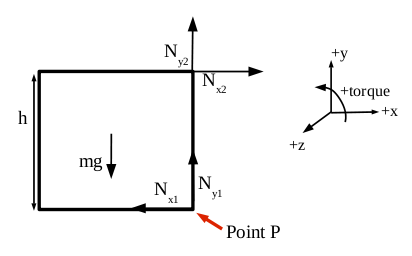
\includegraphics[width=0.7\textwidth]{figures/exam4problem1partA.png}
	\caption{force diagram of square sign and coordinate system}
	\label{fig:forceDiagram}
\end{figure}

b.the net torque at any point must be zero, and the net force in each direction must be zero \newline
m = mass of sign, h = length of one side on the sign\newline
net force in the x direction: $0 = N_{x2} - N_{x1}$\newline
net force in the y direction: $0 = N_{y2} + N_{y1} - mg$\newline
reaction forces in the y direction: $N_{y2} = N_{y1}$\newline
net torque about point P: $0 = \frac{mgh}{2} - N_{x2}h$\newline

c. sign weight = 98. N in -y direction, $N_{x2} = 49.$ N in x direction\newline
$N_{x1} = 49.$ N in -x direction, $N_{y1} and N_{y2} = 49.$ N in y direction\newline
about point P, the weight creates a torque of 20. Nm in the -z direction\newline
about point P, the reaction force $N_{x2}$ creates a torque of 20. Nm in the z direction\newline

sign mass m = 10.0 kg, g = 9.8 $\frac{m}{s^{2}}$, h = 0.40 meters\newline
solving the equations from part b yields\newline
torque about point P: $0 = \frac{mgh}{2} - N_{x2}h \rightarrow N_{x2} = \frac{mg}{2}$\newline
thus $N_{x1} = \frac{mg}{2}$ in -x direction\newline
net force in y direction $\rightarrow N_{y1} = N_{y2} = \frac{mg}{2}$
%%%%%%%%%%%%%%%%%%%%%%%%%%%%%%%%%%%%%%%%%%%%%%%%%%%%%%%%%%%%%%%%%%%%%%%%%%%%%%%%
